\documentclass{article}


% if you need to pass options to natbib, use, e.g.:
%     \PassOptionsToPackage{numbers, compress}{natbib}
% before loading neurips_2021

% ready for submission
\PassOptionsToPackage{numbers, compress}{natbib}
\usepackage[preprint]{neurips_2021}
\bibliographystyle{abbrvnat}

\usepackage[utf8]{inputenc} % allow utf-8 input
\usepackage[T1]{fontenc}    % use 8-bit T1 fonts
\usepackage[colorlinks=true]{hyperref}       % hyperlinks
\usepackage{url}            % simple URL typesetting
\usepackage{booktabs}       % professional-quality tables
\usepackage{amsfonts}       % blackboard math symbols
\usepackage{nicefrac}       % compact symbols for 1/2, etc.
\usepackage{microtype}      % microtypography
\usepackage{xcolor}         % colors
\usepackage{siunitx}
\usepackage{graphicx}

\newcommand{\todo}[1]{{\color{red}todo: #1}}

\title{Spotify feat. Logistic Regression - \\ Popularity, Nothing Else Matters}

% The \author macro works with any number of authors. There are two commands
% used to separate the names and addresses of multiple authors: \And and \AND.
%
% Using \And between authors leaves it to LaTeX to determine where to break the
% lines. Using \AND forces a line break at that point. So, if LaTeX puts 3 of 4
% authors names on the first line, and the last on the second line, try using
% \AND instead of \And before the third author name.

\author{%
  Sebastian Hoffmann\thanks{correspondence to \texttt{sebastian.hoffmann@student.uni-tuebingen.de}}\\
  University of Tübingen\\
  Matriculation number 5954377\\
  \And
  Yannick Streicher\thanks{correspondence to \texttt{yannick.streicher@student.uni-tuebingen.de}}\\
  University of Tübingen\\
  Matriculation number 5331817\\
}

\begin{document}

\maketitle

\begin{abstract}
  What is the musical taste of the world? With the recent rise and global pervasiveness of music streaming services, such as Spotify, Deezer, or Apple Music, answering this question has become tractable. For this, we plan to analyze a \href{https://www.kaggle.com/rodolfofigueroa/spotify-12m-songs}{subset of 1.2 million songs} scraped from Spotify. However, this dataset lacks crucial information about popularity. Thus, an important step of our work is to augment the dataset further by querying the official Spotify REST API for a randomly sampled subset of the data. Besides a birds-eye overview of the musical landscape, e.g. distribution of genres, we want to identify common musical properties shared by popular songs, and likewise, very unpopular songs, using logistic regression. Such properties can be, for instance, tempo, mode, or key.
\end{abstract}

\section{Introduction}

%With the recent advent of musical streaming services, such as Spotify, or Apple Music, unprecedented amounts of data became readily available to a public audience. This data can often be accessed free-of-charge using an API provided by the service provider itself.


%% general overview - i) we want dataset and clusters, ii) we want to predict popularity
%The large amount of digital music today can be daunting. To successfully navigate this space, we urgently need better knowledge of the key characteristics of this opaque, highdimensional space.

With our work, we want to present two important findings that contribute to this goal in a twofold manner: \textit{First} we create a clear overview of the musical landscape. That is, by applying t-SNE (\todo{cite?}) we show a twodimensional embedding of the high dimensional space of audio tracks. We find clusters that can be labeled as musical \textit{genres}. \textit{Second}, we zoom in and, using logistic regression, distill audio features that are of particular interest when considering the popularity of an audio track.

% motivation for the data: aggregate popularity measures with audio features
% or, we are guided by spots popularity measure
To predict the popularity of a song given its Spotify features, we have to find good labels that discriminate popular and unpopular songs.
To measure users responses to individual songs, Spotify presents two metrics, \textit{(i): Popularity:} An algorithmically determined integer between 0 and 100 (more is better), based on the total number of (recent) plays a track has. Artist popularity is derived from the popularity of its individual tracks. The second feature is \textit{(ii): Followers} which is the number of accounts that subscribed to this artists Spotify feed. The number can be interpreted as peoples interest in following the new releases of a particular artist.

\section{Dataset}
\label{sec:dataset}

While Spotify provides data about individual songs or artists via its API, it does, however, not provide a catalogue of available songs on its platform. Thus, we use a dataset\footnote{\url{https://www.kaggle.com/rodolfofigueroa/spotify-12m-songs}} of $1.2$ million songs made available on Kaggle, a subset of the $70$ million songs accessible on Spotify~\cite{ingham_2020}. This dataset was created by first downloading the \href{https://musicbrainz.org/}{MusicBrainz} catalogue, an open-collaboration database of music releases, and then querying the Spotify API. 

For each song listed, the dataset contains basic meta informations such as artist and song name, as well as a set of $14$ song features that are provided by Spotify. These features include, among others, the estimated tempo, key, \emph{energy}, \emph{danceability}, or duration of the song. For a full list, refer to the Spotify API documentation. Crucially, the \emph{popularity} or genre of a song is not included in this dataset.

\subsection{Augmentation}
In a first step we retrieve additional information of all \num{85 113} artists appearing in the dataset from the Spotify API. This information includes the popularity of that artist, aggregated from individual songs, the number of followers, and optionally a list of genres the artist is associated with.

Additionally, we query the Spotify API for every song in the dataset to obtain its individual popularity. While Spotify does not provide genre information at song level, we use the genre information associated with the first artist to further augment the dataset. The exact procedure is described in Section~\ref{sec:genre_clustering}. 

\subsection{Filtering}

%\begin{figure}[t]
%  \centering
%  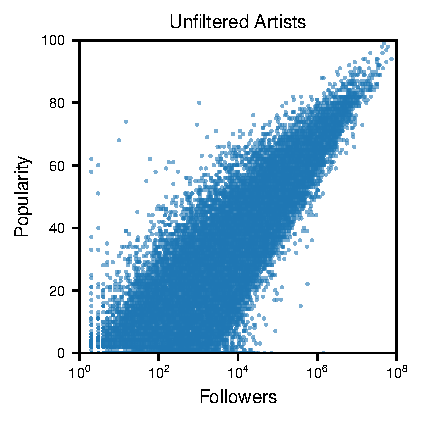
\includegraphics[width=0.38\textwidth]{../figures/artists_unfiltered.pdf}
%  \qquad
%  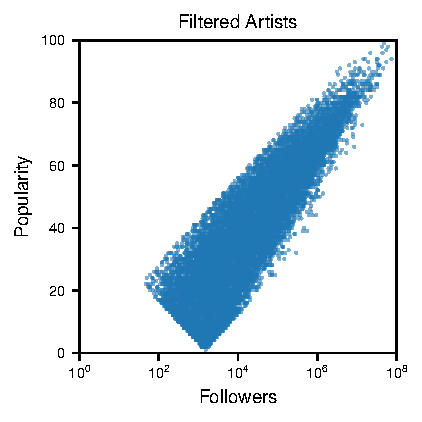
\includegraphics[width=0.38\textwidth]{../figures/artists_filtered.pdf}
%  \caption{\textit{Left}: Artist popularity against log-followers before applying our filtering rules. \textit{Right}: We use the result of PCA to exclude artists that are outliers with respect to the first and second principal component.}
%  \label{fig:filtering}
%\end{figure}

To reduce potential noise introduced by unknown self-published artists, we want to restrict our analysis to those that can be considered professional or semi-professional musicians. This step was deemed necessary, as self-published artists do not undergo the feedback and quality control process a regular music label would provide. Indeed, we find that a quarter of artists on Spotify have less than $45$ followers and half of all artist have less than $393$.
%For comparison, \emph{Merikan}, a relatively unknown Drum and Bass producer, has $4581$ follower at the time of writing.

We find that the number of followers is roughly exponentially distributed. After applying a logarithmic transform, a clear linear relationship between the number of log-followers and popularity is visible (Pearson correlation coefficient: $0.88$, c.f. Fig.~\ref{fig:filtering},~left). 

Based on the popularity and log-follower count, we derive a robust filter criterion using principal component analysis~(PCA)~\cite{jolliffe2016principal}. After applying PCA, the first principal component is treated as a measure of the successfulness of an artist, taking both his popularity and followers into account. We threshold this measure to only include $50\%$ of all artists. Furthermore, we threshold the second component as well to remove outliers, i.e. artists with a high discrepancy between popularity and follower count. This step affects $1.6\%$ of all artists. Finally, we exclude those without associated genres.

In total, if all three steps are applied, $62.8\%$ of all artists are removed from the dataset. This reduces the number of songs left in the dataset to $755472$ ($62.75\%$).

\subsection{Finding metagenres by clustering}
\label{sec:genre_clustering}
The genres associated with an artist are often very fine-granulated. Out of \todo{$111$} genres in total, only \todo{$111$} have more than \todo{$123$} artists associated with them. To reduce the number of overall genres to a handful of overarching \emph{metagenres}, such as Rock, Jazz, or Hip-Hop, we employ agglomerative clustering~\cite{ward1963hierarchical} (we use~\cite{scikit-learn}). Agglomerative clustering lends itself naturally for this task as it exploits the inherent hierachical relationship between genres.

Inspired by constrastive methods~\cite{mikolov2013efficient, chen2020simple}, we exploit the fact that related genres are more likely to be associated with the same artist to construct a distance measure. In a first step, a similarity measure $s_{i, j} = (2 n_{ij}) / (N_i + N_j)$ between the $i$-th and $j$-th genre is defined, where $n_{ij}$ denotes the number of times they appear together and $N_i, N_j$ the total counts of the $i$-th and $j$-th genre respectively. The distance can then be defined as the reciprocal of that similarity measure. We then use this distance measure for the clustering procedure.

By running the clustering algorithm on an aggressively filtered subset of genres, we find $32$ metagenres, among them Jazz, Classical, Metal, Rock, Pop, or EDM, but also Soundtrack, or Show Tunes\footnote{Metagenres have been manually annotated}. These cover $60.5\%$ of all songs in the filtered dataset. To further improve coverage of songs, we rerun the clustering with less aggressive filtering to include more fine-grained genres. We then manually append these additional subgenres to the appropriate metagenre if applicable. This improves coverage to $71.3\%$.

\section{Experiments}

\subsection{Genre analysis}

\begin{figure}
  \centering
  % 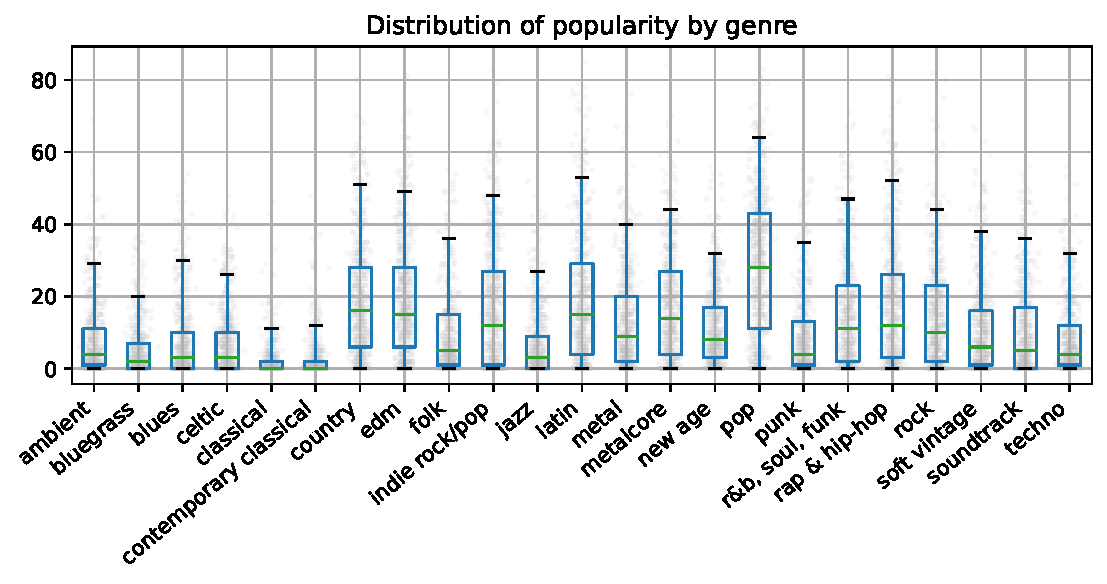
\includegraphics[width=0.85\textwidth]{../figures/popularity_distribution_by_genre.pdf}
  \caption{Box plot of popularity grouped by genre. Boxes span $Q1$ to $Q3$,while whiskers indicate the $5$-th and $95$-th percentile respectively. The central line shows the median of the distribution. Among all genres, Pop has the highest median and $95$-th percentile.}
  \label{fig:genre_boxplot}
\end{figure}

The most prelevant genre on Spotify is Classical ($20.6\%$), followed by Rock ($7.9\%$), Rap / Hip-Hop ($7.6\%$), Metal ($6.3\%$), Folk ($6.0\%$), and Jazz ($4.0\%$). For a full overview, we refer to the supplementary material available on github\footnote{\url{https://github.com/ystreicher/SpotifyNEM2022}}.

The box plot presented in Fig.~\ref{fig:genre_boxplot} shows the distribution of popularity for each genre. We find that despite  being the most prominent genre, Clasical and Contempory Classical are by far the most unpopular with the majority of the probability mass below $10\%$. Notably, Pop has by far the heaviest tails and the highest median and $75$-th percentile of all genres despite only making up $2.9\%$ of all songs. Following after Pop, we find that Country, EDM, Latin, Rock, Indie Pop, Hip-Hop, and Metalcore are almost equally popular.  

Lastly, as a preliminary experiment for the logistic regression, we investigate the discriminative power of the song features provided by Spotify. For this, we embedd the features of songs of the six most popular genres into a two-dimensional vector space using t-SNE~\cite{van2008visualizing} (we use~\cite{Policar731877}). Results are presented in Fig.~\ref{fig:tsne_genres} in the appendix. Clearly visible are distinct cluster of songs corresponding to genres such as Hip-Hop, Metal, Classical or Jazz. Additionally, genres that are arguably related to each other, such as Rock and Metal, or Jazz and Classical, are clustered close together or have some overlap.

\subsection{Logistic Regression}
% implicit assumtion: popularity = f(audio features)
%For this project, the variable of interest is being \textit{popular} vs. \textit{unpopular} for individual tracks.
%For the prediction we consider the \textit{audio features} for each of the tracks. 
We verify whether a linear model is suitable to predict popularity from the audio features (c.f.~Section~\ref{sec:dataset}) by the application of standard linear regression\footnote{\url{https://www.statsmodels.org}}.
The model yields significant but small coefficients that can only explain about \SI{10}{\percent} ($R^2 = 0.105$) of the variance in the data.
The most prominent feature is \emph{loudness} with weight \num{0.027}.
In order to get more insights, we use logistic regression\footnote{\url{https://scikit-learn.org}} to classify songs as either popular or unpopular. 

Binary labels are obtained by thresholding the popularity value of a song. Despite our aggressive filtering, we find that the popularity is roughly exponentially distributed. To deal with such a highly-skewed distribution, we try two thresholding strategies:
\begin{enumerate}
  \item[(A)] Any song with populartiy below the $90$-th percentile is labelled \emph{unpopular}, otherwise as \emph{popular}. To counteract the class-imbalance, the class weights are adjusted as detailed in~\cite{haixiangLearningClassimbalancedData2017a}.
  \item[(B)] The songs are evenly split into two classes at the $50$-th percentile.
\end{enumerate}

In all experiments an 80-20 train-test split is used, and $\ell_2$-regularizaton is employed in both cases. To find the optimal regularization strength, we performed a grid-search using 5-fold cross validation on the training set.

Overall, model A achieves an accuracy of $0.59$, whereas model B achieves an accuracy of $0.62$ w.r.t. to their respective labels.
A calibration plot is presented in Fig.~\ref{fig:logis_eval}~(left). 
Both models fail to deliver a well-calibrated distribution of song-popularity.
Those results, as well as, the low $R^2$ value of the linear regression model could be pointers to insufficient capacity of the linear model class.
However, fitting a Multi-Layer Perceptron (MLP) can only marginally improve the results.

% weight interpretation - elaborate what stood out
Nevertheless, we show learned coefficients of model B in Fig.~\ref{fig:logis_eval} (right). Especially loudness and danceability seem to be indicative of popularity according to the model. In contrast, acousticness, instrumentalness, energy, and valence appear to have a negative impact.

\begin{figure}
  \centering
  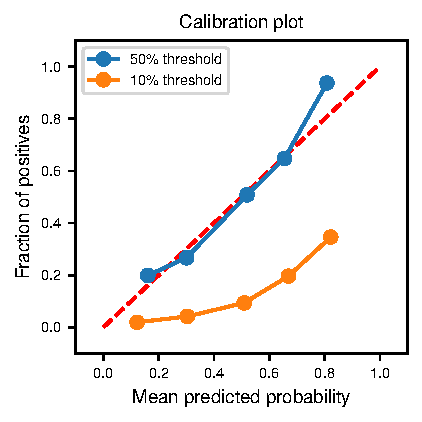
\includegraphics[width=0.39\textwidth]{../figures/calibration_combined.pdf}
  \qquad
  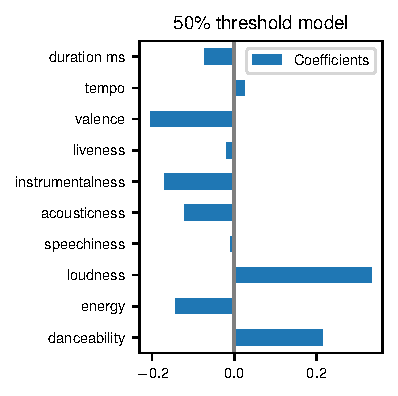
\includegraphics[width=0.39\textwidth]{../figures/logistic_coefs_50_threshold_model.pdf}
  \caption{\textit{Left}: Calibration plot following the methodology of \cite{niculescu-mizilPredictingGoodProbabilities2005}. The prediction space is discretized into \num{20} bins. Using the test set, for each bin, we plot the fraction of true popular songs against the mean predicted probability for those songs. \textit{Right}: The coefficients of the selected model for each audio feature. For the interpretation of individual features consider the API documentation of Spotify.}
  \label{fig:logis_eval}
\end{figure}
  

\section{Conclusion}

In this work, we gave an overview of the musical landscape as seen by Spotify.
We demonstrated that agglomerative clustering can successfully be applied to aggregate the thousands of microgenres identified by Spotify's algorithm into a handful of supergenres. 
Furthermore, we have shown that the musical features provided by Spotify's API are highly discriminative in terms of \emph{musical relatedness}, by applying t-SNE and showing that songs of the same genre are spatially close in  feature space. 
Despite the fact that we can discriminate genres by popularity (see Section~3), linear models fail to robustly classify individual songs as popular or unpopular.

The experiments show that loudness correlates, albeit very weakly, with the popularity of a song. But this does not mean that louder songs are more popular. Rather, it is evidence that more successful tracks often come from high-end production facilities. 
The work allows two conclusions: Either, the crucial factors for popularity are not represented in the data set, or, higher capacity models are needed to solve the problem.


\bibliography{bibliography}

\begin{appendix}
\section{Appendix}

\newpage

\begin{figure}
  \centering
  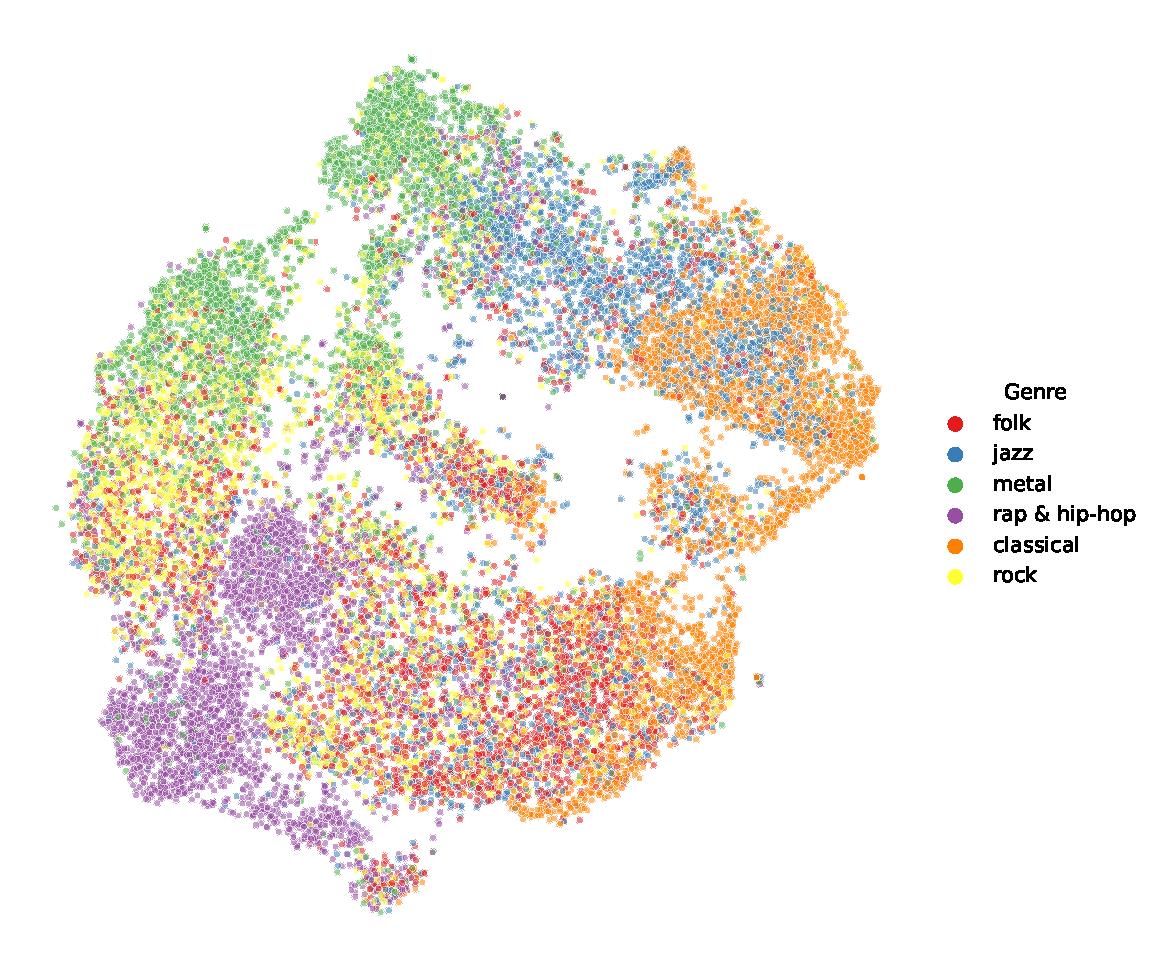
\includegraphics[width=1.0\textwidth]{../figures/tsne_genres.pdf}
  \caption{tsne}
  \label{fig:tsne_genres}
\end{figure}

\end{appendix}

\end{document}
